\epigraph{\textit{``Indeed, brute force is a perfectly good technique in many cases; the real question is, can we use brute force in such a way that we avoid the worst-case behavior?''}}{--- \citeauthor{taocv3}, \citeyear{taocv3} \cite{taocv3}}
Esta solución busca el menor costo para transformar una cadena de caracteres `origen` en otra cadena `objetivo`. Cada operación tiene un costo asignado: la sustitución cuesta 2 si los caracteres son diferentes, la inserción y eliminación cuestan 1, y la transposición cuesta 1. La función `transformar` es recursiva y evalúa todas las posibles transformaciones aplicables en cada posición de las cadenas. Como tal, el programa no transforma el string, sino que calcula directamente el costo de estas operaciones.
\\
El programa ejecuta cada una de las posibilidades para cada caracter del string, ejecutando todas las opciones y eligiendo la menor de estas. En el siguiente ejemplo se revisa un camino optimo en donde vemos el costo de transformar 'plomero' a 'polimeros'

\vspace{1em} % Espacio adicional para separación

\begin{figure}[h]
    \centering
    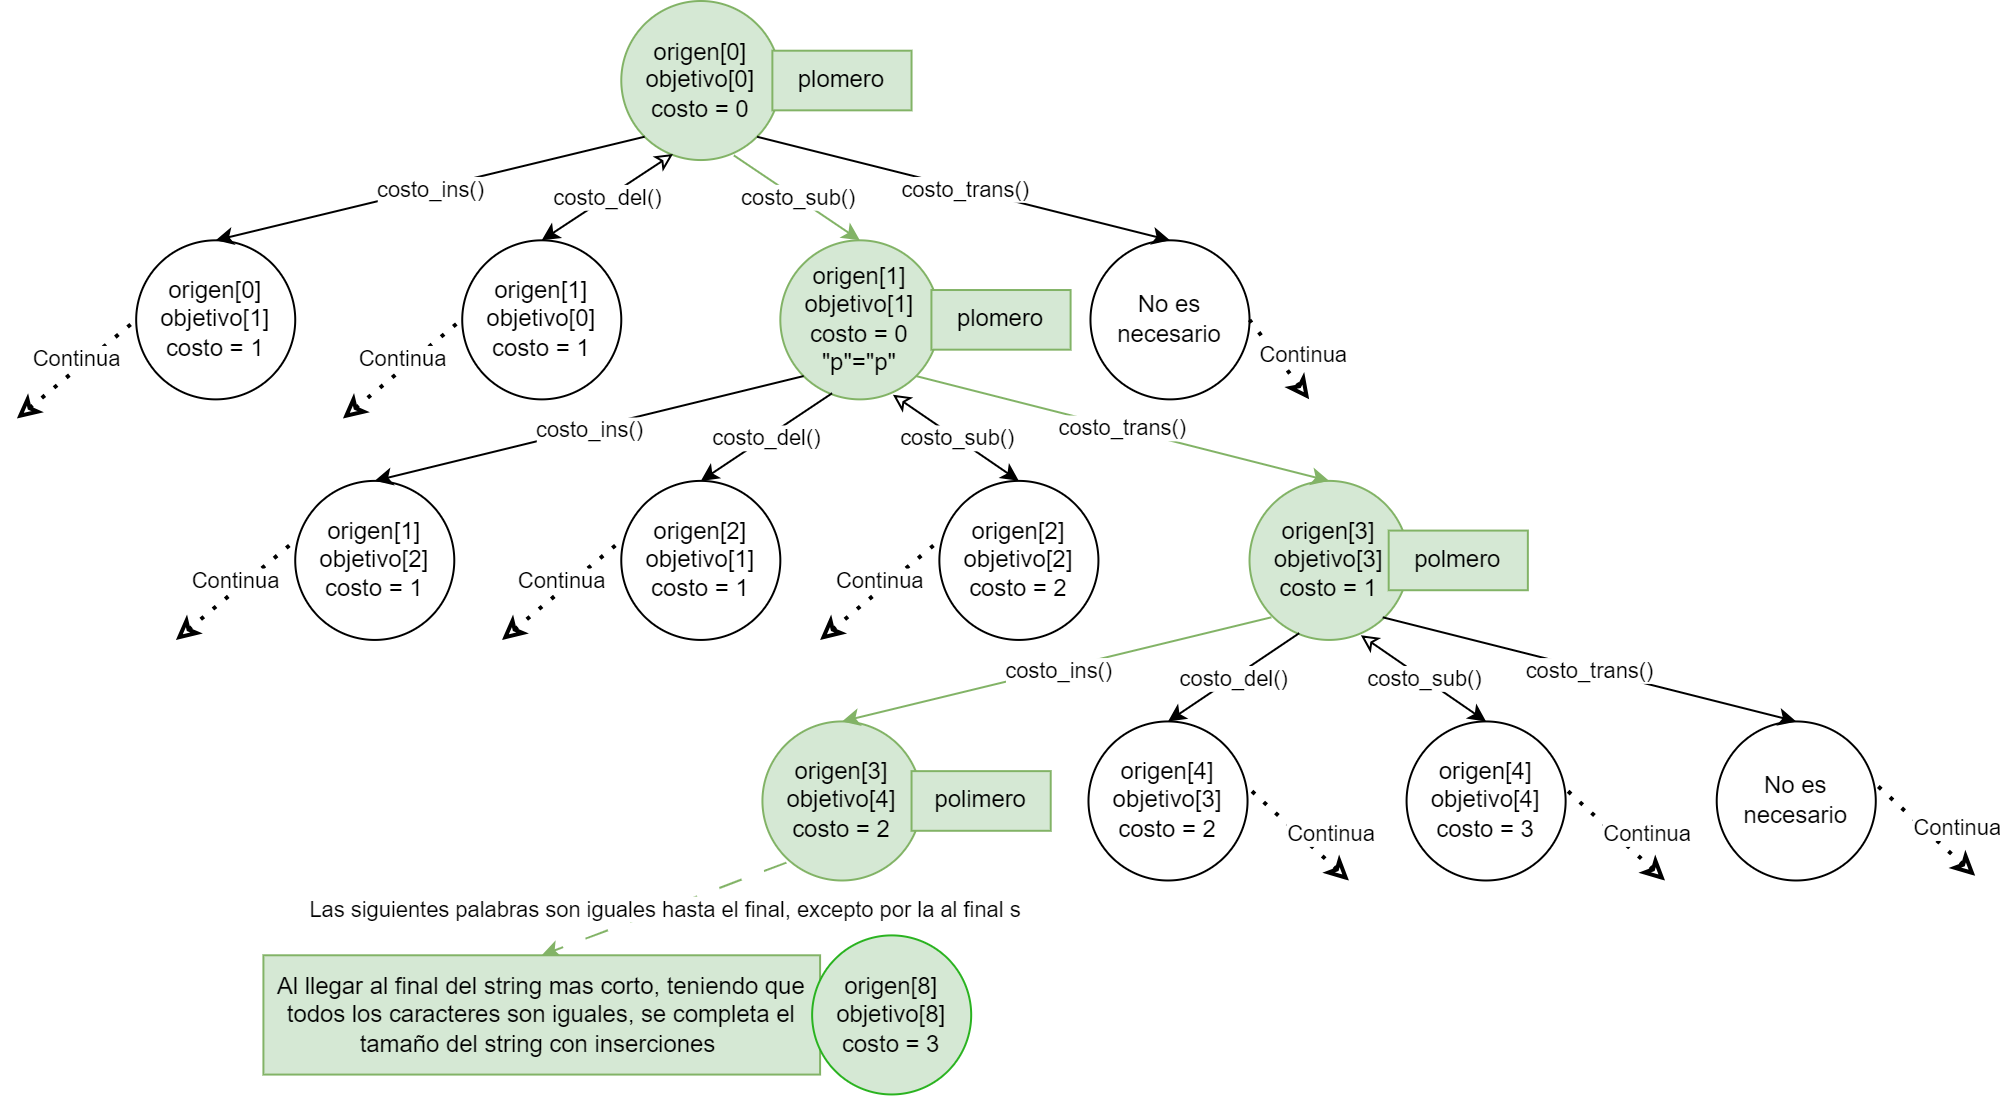
\includegraphics[width=1\linewidth]{AlgoReportTemplate-main/images/Bruteforce Plomero-Polimeros.png}
    \label{fig:enter-label}
\end{figure}
El programa revisa todos los casos posible en el string recursivamente, llegando al ultimo caracter del string, donde retorna en caso de que haya una diferencia en el tamaño del string. cuando llega al nivel mas abajo, comienza a evaluar, retornando el costo de cada transformacion.
\\
\begin{algorithm}[H]
    \SetKwProg{myproc}{Procedure}{}{}
    \SetKwFunction{AlgorithmName}{Transformar}  % Cambia 'AlgorithmName' por el nombre del enfoque elegido
    \SetKwFunction{CostoSub}{costo\_sub}  % Función auxiliar de ejemplo
    \SetKwFunction{CostoIns}{costo\_ins}
    \SetKwFunction{CostoDel}{costo\_del}
    \SetKwFunction{CostoTrans}{costo\_trans}
    \DontPrintSemicolon
    \footnotesize

    % Definición del algoritmo principal
    \myproc{\AlgorithmName{origen, objetivo, i, j, costo\_acumulado}}{
    \uIf{$i =$ longitud de origen y $j =$ longitud de objetivo}{
        \Return costo\_acumulado\;  % Fin de la transformación
    }
    \uElseIf{$i =$ longitud de origen}{
        \Return costo\_acumulado + (longitud de objetivo - $j$)\;  % Coste por inserciones restantes
    }
    \uElseIf{$j =$ longitud de objetivo}{
        \Return costo\_acumulado + (longitud de origen - $i$)\;  % Coste por eliminaciones restantes
    }

    % Caso base: cálculo de costo mínimo
    $costo\_min \leftarrow \infty$\;

    % Costo de sustitución
    $costo\_sust \leftarrow costo\_acumulado + \CostoSub{origen[i], objetivo[j]}$\;
    $costo\_min \leftarrow \min(costo\_min, \AlgorithmName{origen, objetivo, i+1, j+1, costo\_sust})$\;

    % Costo de inserción
    $costo\_inser \leftarrow costo\_acumulado + \CostoIns{objetivo[j]}$\;
    $costo\_min \leftarrow \min(costo\_min, \AlgorithmName{origen, objetivo, i, j+1, costo\_inser})$\;

    % Costo de eliminación
    $costo\_elim \leftarrow costo\_acumulado + \CostoDel{origen[i]}$\;
    $costo\_min \leftarrow \min(costo\_min, \AlgorithmName{origen, objetivo, i+1, j, costo\_elim})$\;

    % Costo de transposición
    \uIf{$i+1 <$ longitud de origen y $j+1 <$ longitud de objetivo y origen[i] = objetivo[j+1] y origen[i+1] = objetivo[j]}{
        $costo\_transp \leftarrow costo\_acumulado + \CostoTrans{origen[i], origen[i+1]}$\;
        $costo\_min \leftarrow \min(costo\_min, \AlgorithmName{origen, objetivo, i+2, j+2, costo\_transp})$\;
    }

    \Return costo\_min\;
}

    % Definición de la función auxiliar
    \myproc{\CostoSub{a, b}}{
    \Return \uIf{$a = b$}{0\;} \Else{2\;}
    }
    
    \myproc{\CostoIns{b}}{
        \Return 1\;
    }
    
    \myproc{\CostoDel{a}}{
        \Return 1\;
    }
    
    \myproc{\CostoTrans{a, b}}{
        \Return \uIf{$a = b$}{0\;} \Else{1\;}
    }
    \caption{Algoritmo de transformación por fuerza bruta entre dos cadenas para encontrar el costo mínimo de conversión. (i y j indices de origen y objetivo, respectivamente)}
    \label{alg:mi_algoritmo_1}

\end{algorithm}
El programa tiene un orden temporal de \(O(4^{\min(m, n)})\), ya que por cada carácter realiza 4 llamadas recursivas, repitiendo el mismo proceso. Al llegar al final del string más corto, devuelve la distancia de diferencia con el otro string. Espacialmente, al pasar los strings por referencia, el orden espacial es \(O(m+n)\).

El programa utiliza recursión en los métodos que alteran el string. La sustitución implica eliminar e insertar un elemento, lo cual tiene un costo acorde. Sin embargo, la transposición introduce una recursión adicional, ya que, aunque pueda implicar una eliminación e inserción en posiciones cercanas, su costo justifica evaluarla.
\newpage